\documentclass[a4paper,11pt]{book}

\usepackage{graphicx}
\usepackage{caption}
\usepackage{subfigure}
\usepackage{fullpage}
%\usepackage{MinionPro}
\usepackage[scaled=.95]{inconsolata}
\usepackage[Sonny]{fncychap}
\usepackage{fancyhdr}
\usepackage{titlesec}
\usepackage{titling}
\usepackage{xcolor}
\usepackage{listings}
\usepackage{multicol}
\usepackage{colortbl}
\usepackage{ifpdf}
\ifpdf
\usepackage[protrusion=true,expansion=true]{microtype}
\usepackage{hyperref}
\else
\usepackage{url}
\fi

%\renewcommand{\sfdefault}{Myriad-LF}
\renewcommand{\maketitlehooka}{\sf}
\renewcommand{\captionfont}{\small\it}
\renewcommand{\captionlabelfont}{\sf}
\titleformat*{\section}{\sf\Large}
\titleformat*{\subsection}{\sf\large}

\ChNameVar{\Large\sf}
\ChNumVar{\fontsize{60}{1}\selectfont}
\ChTitleVar{\Huge\sf}
\ChRuleWidth{0pt}
\ChNameAsIs

\arrayrulecolor{tableborder}
\renewcommand{\arraystretch}{1.5}
\setlength{\arrayrulewidth}{0.5pt}

\pagestyle{fancy}

\definecolor{lightgray}{RGB}{240,240,240}
\definecolor{darkgray}{RGB}{100,100,100}

\definecolor{tableborder}{RGB}{0,0,0}
\definecolor{tableheader}{RGB}{192,192,193}
\definecolor{tablerow}{RGB}{238,238,238}
\definecolor{tablegray}{RGB}{228,228,230}
\definecolor{tableorange}{RGB}{255,204,50}

\definecolor{hyperrefcite}{RGB}{0,51,153}
\definecolor{hyperrefurl}{RGB}{153,51,51}

\definecolor{codelinenumber}{RGB}{43,145,175}
\definecolor{codekeyword}{RGB}{0,0,255}
\definecolor{codecomment}{RGB}{0,128,0}
\definecolor{codestring}{RGB}{163,21,21}

\lstset{
    basicstyle=\ttfamily\small,
    commentstyle=\color{codecomment},
    stringstyle=\color{codestring},
    keywordstyle=\color{codekeyword},
    xleftmargin=5px,
    xrightmargin=5px,
    framexleftmargin=5px,
    framexrightmargin=5px,
    frame=single,
    backgroundcolor=\color{lightgray},
    rulecolor=\color{tableborder},
    lineskip=-1px,
    showstringspaces=false,
    fontadjust
}

\ifpdf
\hypersetup{
    bookmarks=true,
    unicode=false,
    pdftoolbar=true,
    pdfmenubar=true,
    pdffitwindow=false,
    pdfstartview={FitV},
    pdfpagelayout={TwoPageRight},
    pdftitle={Network Laboratory},
    pdfauthor={Ruizhi Liao, Alex Bikfalvi, Jaume Barcelo, Albert Rabassa},
    pdfsubject={Lab practice},
    pdfcreator={LaTeX2e},
    pdfproducer={Universitat Pompeu Fabra},
    pdfkeywords={traffic} {analysis} {LAN} {WLAN} {VLAN} {STP},
    pdfnewwindow=true,
    colorlinks=true,
    linkcolor=black,
    citecolor=hyperrefcite,
    filecolor=black,
    urlcolor=hyperrefurl
}
\fi

\begin{document}

\frontmatter
\pagestyle{empty}

\begin{titlepage}
\begin{center}

%\Huge Network Laboratory
%\author{}
%
%\maketitle

\ifpdf

\includegraphics[width=0.3\linewidth]{Figures/Logo.pdf}\\[9cm]
\else

\includegraphics[width=0.3\linewidth]{Figures/Logo.eps}\\[9cm]
\fi

\textsf{\Huge Network Laboratory}\\[1cm]

\textsf{Ruizhi Liao, Alex Bikfalvi, Jaume Barcelo, Albert Rabassa}\\[1cm]

\textsf{Spring 2013}

\vfill

\textsf{Last updated: \today}

\end{center}
\end{titlepage}

\tableofcontents

\mainmatter

\input{About}
\chapter{Traffic Analysis}

\section{Introduction}

The goal of this lab assignment is to learn about monitoring and traffic analysis tools. We shall use the \emph{Wireshark} and \emph{tcpdump} software tools to study different layers of the TCP/IP architecture.

\section{Home Preparation}

Review the TCP/IP model and explain the function of each layer. Provide examples of the protocols at each layer of the protocol stack.

\begin{center}
\sffamily\small
\begin{tabular}{>{\columncolor{tablegray}}p{15cm}}

\multicolumn{1}{>{\columncolor{tableorange}}l}{Questions and Tasks}\\
What is the purpose of ARP? \emph{Tip: Use the RFC826 standard to answer this question \cite{rfc826}.}\\
\hline
Draw a sketch of the different messages being exchanged and the different steps involved.\\
\hline
Is it possible to run this protocol between computers that are in different local area networks (LANs)?\\
\hline
What is the ICMP protocol?\\
\hline
How does the \emph{ping} command work?\\
\hline
What does the \emph{ping} command measure?\\
\hline
Explain and draw an SSL connection indicating how the protocol works and which messages are being exchanged.\\
\hline
\end{tabular}
\end{center}

\section{Disable Your Local Firewall}

On a Linux machine, your local firewall can interfere with the assignment. Disable it using the following command with root permissions.

\begin{lstlisting}
service iptables stop
\end{lstlisting}

\section{Wireshark Network Analyzer}

Start your computer in Linux. Start the \emph{Wireshark} software program and choose the correct network interface from the \textbf{\sf Capture} \textgreater \textbf{\sf Interfaces} dialog. Use it to start the packet capture. It is also possible to configure the length of the capture and other details.

\begin{center}
\sffamily\small
\begin{tabular}{>{\columncolor{tablegray}}p{15cm}}

\multicolumn{1}{>{\columncolor{tableorange}}l}{Questions}\\
What interface does Wireshark detect? What is your IP address? What is the corresponding MAC address?\\
\hline
\end{tabular}
\end{center}

Configure the \textbf{\sf Capture} \textgreater \textbf{\sf Interfaces} options to perform a five minutes capture. Observe the results and answer the following questions.

\begin{center}
\sffamily\small
\begin{tabular}{>{\columncolor{tablegray}}p{15cm}}

\multicolumn{1}{>{\columncolor{tableorange}}l}{Questions}\\
What is the total number of captured packets? Are there lost packets? If yes, why?\\
\hline
\end{tabular}
\end{center}

Select a (any) packet. Observe the details and answer the following questions.

\begin{center}
\sffamily\small
\begin{tabular}{>{\columncolor{tablegray}}p{15cm}}

\multicolumn{1}{>{\columncolor{tableorange}}l}{Questions}\\
What is the source and destination IP address?\\
\hline
What are the source and destination MAC addresses?\\
\hline
What is the number of bytes in the packet?\\
\hline
What protocols can you see in the packet?\\
\hline
Did you capture an HTTP packet? If yes, what is the length of the HTTP message (the payload of the TCP segment or segments)?\\
\hline
What are the source and destination port?\\
\hline
\end{tabular}
\end{center}

In the dialog \textbf{\sf Analyze} \textgreater \textbf{\sf Enable Protocols...} you can configure the protocols that Wireshark captures and displays. Looking at the default protocols, find at least one protocol of each of the four upper layers of the TCP/IP stack (application, transport, internet and link). Include a brief description of the protocols you found.

Select the menu \textbf{\sf Statistics} \textgreater \textbf{\sf Protocol Hierarchy} and observe the percentage of the following protocols: Ethernet, Internet Protocol, TCP, UDP, Logical Link Control, ARP, STP, IPv6, HTTP.

Repeat the previous capture using IPv6, by performing ping to the local-link IPv6 address of a neighbor or attempting an IPv6 ping to an existing destination. You may use one of the following commands:

\begin{lstlisting}
ping6 -I <interface> <address>
\end{lstlisting}
or:
\begin{lstlisting}
ping6 ipv6.google.com
\end{lstlisting}

\begin{center}
\sffamily\small
\begin{tabular}{>{\columncolor{tablegray}}p{15cm}}

\multicolumn{1}{>{\columncolor{tableorange}}l}{Questions}\\
What are the differences between IPv4 and IPv6?\\
\hline
\end{tabular}
\end{center}

\section{The Address Resolution Protocol (ARP)}

The Address Resolution Protocol (ARP) resolves the association between an IP address and a MAC address. It is used in IP over Ethernet networks. Begin a new traffic capture and analyze the ARP packets. You can filter the ARP packets by writing \texttt{\color{blue}ARP} in the \textbf{\sf Filter Toolbar}.

If you do not capture any ARP packets, clear your ARP cache and then ping or browse to any preferred destination. You can use the following command to delete all ARP entries. On a Windows computer use.

\begin{lstlisting}
arp -d *
\end{lstlisting}
On a Linux computer use.

\begin{lstlisting}
sudo ip neighbour flush all
\end{lstlisting}

\begin{center}
\sffamily\small
\begin{tabular}{>{\columncolor{tablegray}}p{15cm}}

\multicolumn{1}{>{\columncolor{tableorange}}l}{Questions}\\
What are the source and destination MAC addresses of the Ethernet frame that contains the ARP request message?\\
\hline
What are the source and destination IP addresses in the ARP request and response frames?\\
\hline
What are the source and destination MAC addresses in the ARP request and response frames?\\
\hline
What is the time elapsing between an ARP request and reply messages?\\
\hline
\end{tabular}
\end{center}

Use the information available in \emph{Wireshark} to indicate the length of the ARP frames and draw the format of the messages.

\begin{center}
\sffamily\small
\begin{tabular}{>{\columncolor{tablegray}}p{15cm}}

\multicolumn{1}{>{\columncolor{tableorange}}l}{Question}\\
To which layer does ARP belong?\\
\hline
\end{tabular}
\end{center}

\section{HTTP and Secure HTTP}

Begin a new 5 minutes capture and during this time visit a few web sites, such as \url{http://www.upf.edu} and \url{https://www.google.com}. After the capture finishes, observe the HTTP and HTTPS messages by typing \texttt{\color{blue}http or ssl} in the filter toolbar. Observe an HTTP GET message and the corresponding response and answer the following questions.

\begin{center}
\sffamily\small
\begin{tabular}{>{\columncolor{tablegray}}p{15cm}}

\multicolumn{1}{>{\columncolor{tableorange}}l}{Questions}\\
What is the HTTP version of your web browser?\\
\hline
What is the HTTP version of the server?\\
\hline
What language does the client request to the server?\\
\hline
Is it possible to find which are the URLs visited by the user?\\
\hline
At which layer is this information available?\\
\hline
\end{tabular}
\end{center}

The default destination port for web is 80 or 8080, when using a web proxy.

\begin{center}
\sffamily\small
\begin{tabular}{>{\columncolor{tablegray}}p{15cm}}

\multicolumn{1}{>{\columncolor{tableorange}}l}{Questions}\\
What is the source port of the get requests?\\
\hline
Write the source port number for different connections. At which layer can you find this information?\\
\hline
\end{tabular}
\end{center}

Find a DNS query--response message pair. Use \texttt{\color{blue} dns} in the \emph{Wireshark} filter.

\begin{center}
\sffamily\small
\begin{tabular}{>{\columncolor{tablegray}}p{15cm}}

\multicolumn{1}{>{\columncolor{tableorange}}l}{Question}\\
What is the function of DNS?\\
\hline
\end{tabular}
\end{center}

Use the option \textbf{\sf Analyze} \textgreater \textbf{\sf Follow TCP Stream} to analyze a TCP session. Identify the three-way handshake and the session tear-down.

\begin{center}
\sffamily\small
\begin{tabular}{>{\columncolor{tablegray}}p{15cm}}

\multicolumn{1}{>{\columncolor{tableorange}}l}{Question}\\
When using HTTP, it is possible to observe the contents of the web using Wireshark?\\
\hline
\end{tabular}
\end{center}

Now use HTTPS.

\begin{center}
\sffamily\small
\begin{tabular}{>{\columncolor{tablegray}}p{15cm}}

\multicolumn{1}{>{\columncolor{tableorange}}l}{Question}\\
Is it still possible to read the information that is being transmitted? \emph{Tip: Search for SSL packets.}\\
\hline
\end{tabular}
\end{center}

Identify a SSL handshake in \emph{Wireshark}.

\section{ICMP Ping Packet Capture (Homework)}

Close all applications that use the network and \texttt{ping} four different web sites on four different continents. Analyze the results.

\begin{center}
\sffamily\small
\begin{tabular}{>{\columncolor{tablegray}}p{15cm}}

\multicolumn{1}{>{\columncolor{tableorange}}l}{Question}\\
What are protocols used?\\
\hline
\end{tabular}
\end{center}

Draw a frame and explain how the different packet are encapsulated in each other.

\begin{center}
\sffamily\small
\begin{tabular}{>{\columncolor{tablegray}}p{15cm}}

\multicolumn{1}{>{\columncolor{tableorange}}l}{Question}\\
How many ping messages are transmitted by default?\\
\hline
\end{tabular}
\end{center}

Prepare a table with the source, destination, and average packet delay  of the four different ping experiments.

\begin{center}
\sffamily\small
\begin{tabular}{>{\columncolor{tablegray}}p{15cm}}

\multicolumn{1}{>{\columncolor{tableorange}}l}{Questions}\\
What is the packet length?\\
\hline
At which layers can we find source and destination addresses?\\
\hline
What are the addresses types?\\
\hline
Are the ping ICMP query packets sent at constant time intervals in time?\\
\hline
What about the ICMP replies?\\
\hline
What are the reasons for different inter-arrival times for the ICMP reply?\\
\hline
What information is included in the data field of the ICMP packets?\\
\hline
What about in the reply messages?\\
\hline
\end{tabular}
\end{center}

\section{\texttt{tcpdump}}

In this section, we shall use the \texttt{\color{blue}tcpdump} command in Linux. Use:

\begin{lstlisting}
man tcpdump
\end{lstlisting}
to learn about the different parameters and options of this command. With \texttt{\color{blue}tcpdump} it is also possible to filter the traffic according to the source or destination addresses, protocol, port number, etc.

Open a terminal and begin a new \texttt{\color{blue}tcpdump} capture. Enter the \textbf{\sf Ctrl+C} keys to finish the capture.

\begin{center}
\sffamily\small
\begin{tabular}{>{\columncolor{tablegray}}p{15cm}}

\multicolumn{1}{>{\columncolor{tableorange}}l}{Questions}\\
What is the information provided by \texttt{tcpdump} and what is the format used?\\
\hline
To which network layer does the information belong? \emph{Tip: Remember that you can redirect the output to a file using the following command \texttt{\color{blue}tcpdump \textgreater file\_name}}.\\
\hline
\end{tabular}
\end{center}

The first line of \texttt{tcpdump} specifies the network interface used during the capture. To change it, use the \texttt{\color{blue}-i} option.

\begin{center}
\sffamily\small
\begin{tabular}{>{\columncolor{tablegray}}p{15cm}}

\multicolumn{1}{>{\columncolor{tableorange}}l}{Question}\\
What is the interface that you are using?\\
\hline
\end{tabular}
\end{center}

Describe the information provided for the ARP protocol using the following command.

\begin{lstlisting}
tcpdump arp
\end{lstlisting}
Then, execute the same command again using the \texttt{\color{blue}-e} option.

\begin{center}
\sffamily\small
\begin{tabular}{>{\columncolor{tablegray}}p{15cm}}

\multicolumn{1}{>{\columncolor{tableorange}}l}{Question}\\
What is the difference with respect to the previous execution? \emph{Tip: Use the \texttt{tcpdump} manual, if necessary.}\\
\hline
\end{tabular}
\end{center}

Try several new captures related to this assignment, such as

\begin{lstlisting}
tcpdump stp
tcpdump http
tcpdump udp
tcpdump ssl
tcpdump ip
\end{lstlisting}
Try also to make captures for a specific IP address.

\chapter{LAN and WLAN}

\section{Home Preparation}

Connect to the web configuration interface of your home access point and find:
\begin{itemize}
\item The name of the wireless network (SSID or ESSID).
\item Frequency channel.
\item PHY layer data rates.
\item Supported security protocols.
\item Possibility of QoS differentiation.
\end{itemize}

Do a survey and find the information of available wireless networks (name, channel, security settings). On a Windows computer, you can use NetStumbler, whereas on Linux computer you can use the following command:

\begin{lstlisting}
sudo iwlist <wlan_interface> scan
\end{lstlisting}

\section{Equipment}

Each group requires at least \emph{two} (2) computers. However, if possible, \emph{three} (3) computers are better than two. Start one computer in Windows and the other one in Linux. The hardware we shall use during this lab is the \emph{Cisco Aironet 1200} access point. The firmware of the access point is \emph{CISCO IOS Version 12.3(8)JA2}, and you can download the corresponding at the following link:

\url{http://www.jaumebarcelo.info/teaching/lxs/wlan/WLAN_manual.pdf}

To test copying a file across the wireless network, install an FTP server on one of the computers, such as \emph{Filezilla} in Windows and \emph{vsftpd} in Linux. You may use a web browser as an FTP client.

\begin{itemize}

\item On Windows, install and open \emph{Filezilla}, and connect locally from the same PC using the \emph{loopback} interface 127.0.0.1. Create a new user (username \texttt{\color{blue}test} and password \texttt{\color{blue}test}) and share a local folder with several large files. Do not forget to remove the proxy configuration, or select not to use a proxy server for local addresses.

\item On Linux, install \emph{vsftpd} with the following command:
\begin{lstlisting}
sudo yum install vsftpd
\end{lstlisting}
    Once installed, you can find and modify the FTP server configuration in the file \texttt{/etc/vsftpd/vsftpd.conf}. If you need to change the configuration, do not forget to restart the FTP server with the command:
\begin{lstlisting}
sudo services vsftpd restart
\end{lstlisting}
    The server allows by default anonymous access, and therefore you do not need to create a new user. The default shared folder is \texttt{/var/ftp}.
\end{itemize}

\section{Disable Your Local Firewall and Pay Attention to Your Browser}

On a Linux machine, your local firewall can interfere with the assignment. Disable it using the following command:

\begin{lstlisting}
sudo service iptables stop
\end{lstlisting}

If you decide to use \emph{Firefox} to connect to the access point during the assignment, it might be necessary to disable the proxy settings and to uncheck the \emph{offline navigation} option.

\section{Basic LAN Configuration}

Connect the Windows and the Linux computers using a cross-over cable. Check layer-2 connectivity using the LED or the \texttt{\color{blue}mii} command in Linux. Check layer-3 connectivity and measure round-trip time using \texttt{\color{blue}ping}. Configure the interfaces if needed.

Next, you need to estimate the available bandwidth using an FTP file transfer or the \texttt{\color{blue}iperf} tool. Change the Ethernet connection speed to 10 Mbps (full duplex) and estimate the bandwidth again.

%{\color{red}I believe the mii tool is obsolete - update? Include instructions on how to change the connection speed in Windows/Linux.}

\begin{center}
\sffamily\small
\begin{tabular}{>{\columncolor{tablegray}}p{15cm}}

\multicolumn{1}{>{\columncolor{tableorange}}l}{Questions}\\
Is the maximum transmission speed reached? Why?\\
\hline
\end{tabular}
\end{center}

\section{WLAN Basic Configuration}

WLANs can be used as an access point (AP) to LANs. They can also be used to interconnect to LANs using wireless distribution system (WDS). 
WDS can also be used to extend the coverage of a WLAN with access points that don't have a wired connection.
IEEE 802.11 headers can accommodate up to 4 addresses to differentiate between final addresses and per-hop addresses\footnote{This is explained in the theory session}.


First connect the AP to the Windows computer. You may use either a direct connection or a connection using the patch panel. The address is available on the AP, and the administrator user is \texttt{\color{blue}Cisco} and the password is \texttt{\color{blue}Cisco}.

Use the express set-up to configure the AP with the following settings.

\begin{center}
\sffamily\small
\begin{tabular}{>{\columncolor{tablegray}}ll}

\multicolumn{1}{>{\columncolor{tableorange}}c}{Setting} & \multicolumn{1}{>{\columncolor{tableheader}}c}{Value}\\
AP Name & \texttt{LABXARXES\_GRUP\_XX} \\
\hline
SSID & \texttt{grupXX} \\
\hline
Channel & default \\
\hline
Transmit power & default \\
\hline
\end{tabular}
\end{center}

After completing the configuration, verify that the radio interface is up. Indicate what are the security options available. Try different settings and configurations and then connect the AP to the laboratory switch.

Plug-in the WiFi interface into the Linux computer and connect the computer to the AP that you have just configured. Disable the wired interface in order to make sure that you are using the wireless interface. Check that you have network connectivity and use the \texttt{\color{blue}ipconfig} (on Windows) or \texttt{\color{blue}ifconfig} (on Linux) commands to look at the interface configuration. If you have network connectivity, you should be able to ping the other computers of your group (the ones with wired connection) and also be able to connect to the Internet.

Perform measurements from the wireless computer to the wired one and the other way around. Measure the round-trip-time using \texttt{\color{blue}}ping. Measure the throughput using FTP to transfer a large file.

\begin{center}
\sffamily\small
\begin{tabular}{>{\columncolor{tablegray}}p{15cm}}

\multicolumn{1}{>{\columncolor{tableorange}}l}{Questions and Tasks}\\
Can you reach the PHY rate maximum throughput? Why?\\
\hline
Do you observe the same values for the uplink and downlink?\\
\hline
Write down any other observations you find interesting.\\
\hline
\end{tabular}
\end{center}

Use either \emph{Netstumbler} or \texttt{\color{blue}iwlist} to detect the available wireless networks. Write down their configuration. Draw a sketch of the computers, access point and other networking devices in your setting.

\section{Hot-Standby}

The hot-standby is a feature to offer high availability. It consists of a backup AP (\emph{AP-standby}) which takes over if the primary AP (\emph{AP-root}) fails.

\emph{During this assignment, collaborate with another group.}

One of the groups will configure the AP-root and the other the AP-standby.
Make sure that you replicate the same configuration (with the exception of the IP address) in both devices: SSID, network mask and security setting.

\begin{itemize}
\item In the \emph{AP-root}, go to \textbf{\sf Network Interfaces} \textgreater \textbf{\sf Radio 802.11g}, and select \textbf{\sf Access Point (Fallback to radio shutdown)}.
\item In the \emph{AP-standby} go to \textbf{\sf Services} \textgreater \textbf{\sf Hot Standby}. Select \textbf{\sf Enable} and specify the MAC address that the AP will be monitoring (the radio interface of the root-AP). If the configuration is correct, you should be able to see the status that will appear below on the screen.
\end{itemize}

Draw a sketch of all the involved network devices and connections and test that it actually works. To test that it is working, disable the radio interface of AP-root from \textbf{\sf Network interfaces} \textgreater \textbf{\sf 802.11g} \textgreater \textbf{\sf Settings}. After the time-out expires, the AP-standby takes over with the same SSID and security settings.

To gather more information about what is happening, you can run ping tests while the takeover takes place. You can also check the logs in the \textbf{\sf Home} page of the AP configuration interface. Finally, you can check the log of the \emph{Filezilla} server.

\begin{center}
\sffamily\small
\begin{tabular}{>{\columncolor{tablegray}}p{15cm}}

\multicolumn{1}{>{\columncolor{tableorange}}l}{Questions}\\
How long does it take for the PC to recover the connection after AP-root's radio is disabled?\\
\hline
Will the user notice that the connection switches from one AP to the other? How?\\
\hline
Do you think that the default time-out setting are appropriate? Why?\\
\hline
How is the network affected if we change this parameters?\\
\hline
\end{tabular}
\end{center}

Now re-enable the radio interface of AP-root. Then, at the AP-standby, click \textbf{\sf Restart}. Check the information that appears in the \textbf{\sf Home} page of the APs to determine to which AP is the client connected. After you have verified that the client is connected to the AP-root device, disconnect the ethernet cable of AP-root.

\begin{center}
\sffamily\small
\begin{tabular}{>{\columncolor{tablegray}}p{15cm}}

\multicolumn{1}{>{\columncolor{tableorange}}l}{Questions}\\
What happens? Does the AP-standby take over? Why?\\
\hline
\end{tabular}
\end{center}

\section{Configuring an AP as a Repeater}

A repeater AP is not connected to the wired LAN. It is situated within the coverage range of another AP to extend the covered area. Similar to the previous exercise, both APs must share the same configuration (with the exception of the IP address). In this exercise, we shall use the previous \emph{AP-standby} as a repeater.

\begin{itemize}
\item In the \emph{AP-root}, select the option \textbf{\sf Role in radio network} and then choose \textbf{\sf Access point}.
\item In the \emph{AP-repeater} (the former \emph{AP-standby}), disable the hot-standby option. Configure the SSID, and at the bottom of the page \textbf{\sf Security} \textgreater \textbf{\sf SSID Manager} select \textbf{\sf Set Infrastructure SSID} and entering the current SSID. In the \textbf{\sf Express Setup}, choose \textbf{\sf Repeater} for the option \textbf{\sf Role in radio network}.
\end{itemize}

After the configuration changes have been completed, your home screen should show the configuration of your network and the repeater, and the clients connected to each AP. Initially, the client computer is probably connected to the \emph{AP-root}.

By selecting the \textbf{\sf Clients} options, you will see the list of associated clients. You can manually de-associate a particular client, in which case the client will automatically re-connect to the repeater.

To verify that the client connects successfully to the other AP, repeat the round-trip time and bandwidth tests that you have performed before. Do the tests while connected to both \emph{AP-root} and \emph{AP-repeater}. Repeat the ping tests while a file is being transferred.

\begin{center}
\sffamily\small
\begin{tabular}{>{\columncolor{tablegray}}p{15cm}}

\multicolumn{1}{>{\columncolor{tableorange}}l}{Question}\\
Can you observe any difference?\\
\hline
\end{tabular}
\end{center}

\input{Vlans}
\input{Stp}
\chapter{Routing}

\section{Home Preparation}

RIP and OSPF are two of the most widely used routing protocols. Find information about these two protocols and compare them. Describe what is the format of a routing table and explain how each of the protocols work.

Read the following quick guide:

\url{www.jaumebarcelo.info/teaching/lxs/routing/GUIA_RAPIDA_CISCO_2010.pdf}

Then, download the router user manuals:

\url{www.jaumebarcelo.info/teaching/lxs/routing/manuals_routers.rar}

\section{First Session}

In this first session each group will work with a router. The goals of this session are:
\begin{itemize}
\item Getting familiar with the configuration method.
\item Configuring the Ethernet interfaces.
\item Observe the RIP protocol in action.
\item Save the configuration in an external TFTP server.
\end{itemize}

Start your computer in Windows. Before disconnecting the computer from the Internet, download the TFTP server from the web site \url{http://tftpd32.jounin.net/}, and save it on one of the computers that you will use to connect to the router.

The routers are connected to each other using the Ethernet interfaces and forming a topology that you will have to determine by yourselves. Use the console connection to connect to the routers (use either \emph{HyperTerminal} or \emph{putty} to open a serial connection at 9600 bps). The COM port number (e.g. COM1, COM2, etc.) depends on your computer configuration\footnote{You can see the name of the local serial ports in the \emph{Device Manager} snap-in. To open the snap-in, click on \textsf{Start} \textgreater \textsf{Run...}, type \texttt{devmgmt.msc} and click \textsf{OK}. The serial ports are listed under the \emph{Ports} branch.}. The escape keystroke to exit the \texttt{ping} command in a router is \textsf{Ctrl-Alt-6}.

\subsection{Checking the Router Status}

Use the console to connect to your router and try the following commands. Prepare a summary of what you can see with each command.

\begin{lstlisting}
show version
show protocols
show interfaces
show processes
show mem
show ip route
show history
\end{lstlisting}

\subsection{Create a Running and Startup Configuration}

Enter the privileged EXEC mode with the command:

\begin{lstlisting}
Router> enable
\end{lstlisting}

and password \texttt{\color{blue}cisco}, and the the global configuration mode

\begin{lstlisting}
Router# configure terminal
\end{lstlisting}

Find the commands to:
\begin{itemize}
\item show and change the router name;
\item debugging mode configuration;
\item send pings from the router, and;
\item activate fair queueing on the ethernet interfaces (e.g. FastEthernet0/0).
\end{itemize}

Use the following commands to show and save the current configuration to the startup configuration from the privileged mode.

\begin{lstlisting}
Router# show running-config
Router# copy running-config startup-config
\end{lstlisting}


\subsection{IP Addresses Configuration}

Go to your physical router equipment and check which interfaces are visible. Use the following command to see what interfaces are available in the router.

\begin{lstlisting}
Router# show interfaces
\end{lstlisting}

Fill in a table that includes:

\begin{itemize}
\item the interface name;
\item the interface MTU;
\item the interface bandwidth, and;
\item the encapsulation protocol.
\end{itemize}

Enter the Ethernet interface configuration mode with the command:

\begin{lstlisting}
Router(config)# interface <interface name>
\end{lstlisting}

Then, set the IP address to 192.168.10.XX, where XX is your group ID plus 10.
Use a /24 network mask.

\begin{center}
\sffamily\small
\begin{tabular}{>{\columncolor{tablegray}}p{15cm}}
\multicolumn{1}{>{\columncolor{tableorange}}l}{Question}\\
What is the command that you have used?\\
\hline
\end{tabular}
\end{center}

Use the command:

\begin{lstlisting}
Router# show interfaces
\end{lstlisting}

to verify the IP address assignment, and enable the interface with the command:

\begin{lstlisting}
Router(config-if)# no shutdown
\end{lstlisting}

Verify the line status and the interface status using the command:

\begin{lstlisting}
Router(config-if)# show protocols
\end{lstlisting}

Use the commands:

\begin{lstlisting}
Router# show cdp neighbors
\end{lstlisting}

and:

\begin{lstlisting}
Router# show cdp neighbors detail
\end{lstlisting}

to see the neighboring Cisco devices.

Write down the information received from the different interfaces.
\begin{itemize}
\item the neighbor identifier;
\item the IP address, and;
\item the port.
\end{itemize}

Use the \texttt{\color{blue}ping} command to test the connectivity to the other routers in the lab and write down the round-trip times and other results that you may consider relevant. Find out which is the network topology and sketch it in a figure.

From your computer, use the \texttt{\color{blue}telnet} command to connect to the router.

\begin{center}
\sffamily\small
\begin{tabular}{>{\columncolor{tablegray}}p{15cm}}
\multicolumn{1}{>{\columncolor{tableorange}}l}{Question}\\
Is it possible to remotely configure a router?\\
\hline
Is login and password required?\\
\hline
Does a console user notice that there is an ongoing telnet connection?\\
\hline
Use telnet to change a parameter of the router (e.g., the name) and verify the changes both using the console and the telnet connection. What happens?\\
\hline
Do messages appear on the console when changes are done over Telnet? What information is included in these messages?\\
\hline
\end{tabular}
\end{center}

Logout the Telnet session to the Cisco router.

\subsection{IP Routing Configuration}

In this exercise, we shall enable the RIP protocol and check the status of the routing table as well as the RIP transactions of each router.

Check whether IP routing is enabled using the command:

\begin{lstlisting}
Router# show protocols
\end{lstlisting}

\begin{center}
\sffamily\small
\begin{tabular}{>{\columncolor{tablegray}}p{15cm}}
\multicolumn{1}{>{\columncolor{tableorange}}l}{Question}\\
What is the status of IP routing?\\
\hline
\end{tabular}
\end{center}

Enter the global configuration mode and enter the submenu \texttt{\color{blue}router}.

\begin{center}
\sffamily\small
\begin{tabular}{>{\columncolor{tablegray}}p{15cm}}
\multicolumn{1}{>{\columncolor{tableorange}}l}{Question}\\
What is the purpose of this submenu?\\
\hline
\end{tabular}
\end{center}

Use the \texttt{\color{blue}?} command to list available routing protocols and write down the results. Enter into the configuration of RIP.

Use the command:

\begin{lstlisting}
Router(config-router)# network <your network>
\end{lstlisting}

to associate your network to the RIP routing process. Assume that we are working with \emph{C} class IP addresses. Therefore, the last byte of the network address must be 0. Verify that the RIP protocol is now enabled and that your network has been recognized by the router using the command:

\begin{lstlisting}
Router# show ip protocol
\end{lstlisting}

Observe the relevant parameters and answer the following questions:

\begin{center}
\sffamily\small
\begin{tabular}{>{\columncolor{tablegray}}p{15cm}}
\multicolumn{1}{>{\columncolor{tableorange}}l}{Question}\\
What is the use of the timers?\\
\hline
What are their values?\\
\hline
Are they too small, or too large?\\
\hline
What happens if we change the values?\\
\hline
\end{tabular}
\end{center}

Verify the status of the routing table with the command:

\begin{lstlisting}
Router# show ip route
\end{lstlisting}

\begin{center}
\sffamily\small
\begin{tabular}{>{\columncolor{tablegray}}p{15cm}}
\multicolumn{1}{>{\columncolor{tableorange}}l}{Question}\\
What is the meaning of each of the fields in the table?\\
\hline
How can we check which are the networks to which RIP protocols is associated?\\
\hline
If there is no information, why?\\
\hline
\end{tabular}
\end{center}

Work together with another group to do this part. If there is no other group ready, skip this exercise and come back to it when another group reaches this point.

Add an static route to the other group's network. Use the following command from the configuration mode.

\begin{lstlisting}
Router(config)# ip route
\end{lstlisting}

Explain what happens when you use \texttt{\color{blue}traceroute} to the other groups router (both interfaces).  Repeat the experiment after deleting the static route in one of the routers. Explains what happens and why.

The command:

\begin{lstlisting}
Router# debug ip rip
\end{lstlisting}

shows the RIP messages that are sent and received by the router.

\begin{center}
\sffamily\small
\begin{tabular}{>{\columncolor{tablegray}}p{15cm}}
\multicolumn{1}{>{\columncolor{tableorange}}l}{Question}\\
What are the source and destination of these packets?\\
\hline
What information do we obtain?\\
\hline
\end{tabular}
\end{center}

\subsection{Saving the Router Configuration in a TFTP Server}

A convenient way to store a router's configuration is using TFTP. We need to install the TFTP server in a computer with connectivity (layer 3 connectivity) to the router. Install the server and configure in which folder you want to save the router's configuration.

In the router, execute the command:

\begin{lstlisting}
Router# copy running-config tftp
\end{lstlisting}

and follow the instructions to enter the TFT server address (this is one of your computers) and the filename that you want to use. In the computer, open the configuration file using a text editor.

\begin{center}
\sffamily\small
\begin{tabular}{>{\columncolor{tablegray}}p{15cm}}
\multicolumn{1}{>{\columncolor{tableorange}}l}{Question}\\
What can you observe?\\
\hline
\end{tabular}
\end{center}

To copy the configuration in the TFTP server to the router, there are two different options. Either use the command:

\begin{lstlisting}
Router# copy tftp running-config
\end{lstlisting}

on the server or simply copy and paste on the configuration terminal.

\section{Router Interconnection}

In this session, we shall use the WAN (serial) interfaces of the routers. The topology of the network is unknown to us and we have to figure it out. In the previous session we used the Ethernet interfaces to connect the routers, and in this session we will use the serial interfaces.

\subsection{Shutdown the Ethernet Interfaces}

Make sure that there is no cable connected to the Ethernet interface, and that there is a cable connecting the serial interfaces. Delete the IP address of the Ethernet interface:

\begin{lstlisting}
Router(config-if)# no ip address
\end{lstlisting}

and administratively shutdown the interface:

\begin{lstlisting}
Router(config-if)# shutdown
\end{lstlisting}

Verify that the changes have been applied using:

\begin{lstlisting}
Router# show running-config
\end{lstlisting}

\subsection{Configuration of the WAN Serial Interface}

From the privileged EXEC mode of your router, enter the global configuration mode. Enter into the configuration of the WAN serial interface and configure the IP.

To choose the IP, use the following algorithm. Assume the your group id is $X$ and your neighbor's group ID is $Y$. If $X<Y$, then your IP is 192.168.XY.X. Otherwise, it is 192.168.YX.X.

The serial interfaces are interconnected by cables that, in the middle, have male/female connector. The router in the female connector side sets the communication rate. You can find which is the female router issuing the command:

\begin{lstlisting}
Router# show controller
\end{lstlisting}

The DTE interface uses the male connector, and the DCE interface uses the female connector. Alternatively, you may also look at the number on the cable, where 1428 is male and 1429 is female.

Use the command:

\begin{lstlisting}
Router(config-if)# clock rate 128000
\end{lstlisting}

or the closest available rate.

Verify the configuration and use the command:

\begin{lstlisting}
Router(config-if)# no shutdown
\end{lstlisting}

on both connected routers to enable the communication. Then use the command:

\begin{lstlisting}
Router# show protocols
\end{lstlisting}

to verify the state of the line.

Now we will gather information about neighboring devices using the command:

\begin{lstlisting}
Router# show cdp neighbors
\end{lstlisting}

or

\begin{lstlisting}
Router# show cdp neighbors detail
\end{lstlisting}

and we will elaborate a table indicating, for each neighbor, the following information:

\begin{itemize}
\item the neighbor identifier;
\item the neighbor IP address, and;
\item the port.
\end{itemize}

Make sure that routing is enabled using the following commands:

\begin{lstlisting}
Router(config)# ip routing
Router(config)# router rip
Router(config-router)# network 192.168.XX.0
\end{lstlisting}

and look at the routing tables using the command

\begin{lstlisting}
Router# show ip route
\end{lstlisting}

Compare the routing tables to the ones obtained in the previous session and highlight the differences. Use the \texttt{\color{blue}ping} to the other devices in the network.

\begin{center}
\sffamily\small
\begin{tabular}{>{\columncolor{tablegray}}p{15cm}}
\multicolumn{1}{>{\columncolor{tableorange}}l}{Question}\\
Which ones are reachable?\\
\hline
Which ones are not?\\
\hline
Why?\\
\hline
Are there differences in the round-trip-time compared to the measures taken in the previous session?\\
\hline
Why?\\
\hline
\end{tabular}
\end{center}

\subsection{Network Topology}

Prepare a sketch of the network topology that we have used in this session and compare it to the topology of the previous session.

\begin{center}
\sffamily\small
\begin{tabular}{>{\columncolor{tablegray}}p{15cm}}
\multicolumn{1}{>{\columncolor{tableorange}}l}{Question}\\
What are the differences?\\
\hline
What are the advantages?\\
\hline
And disadvantages?\\
\hline
\end{tabular}
\end{center}

\section{Configuration of an L2-L3 Network}

This third session extends the previous one by including switches to the network topology, as shown in the figure~\ref{fig:routers_and_switches}. The topology consists of a ring of routers connected in a ring using the serial interfaces. Each router is connected using the ethernet interface to a local area network with two or more computers. The devices used in this assignment are:

\begin{itemize}
\item computers;
\item up to six Cisco routers with an ethernet interface and two serial interfaces;
\item up to three Cisco switches, and;
\item direct and cross-over RJ-45 cables.
\end{itemize}

\begin{figure}
\centering
\ifpdf
\includegraphics[width=0.9\linewidth]{Figures/routers_and_switches.pdf}
\else
\includegraphics[width=0.9\linewidth]{Figures/routers_and_switches.eps}
\fi
\caption{Network topology that includes routers and switches}
\label{fig:routers_and_switches}
\end{figure}

Each group has to configure its router and its VLAN. It is assumed that the previous session has been successfully completed and the connectivity tests were satisfactory.

\subsection{VLAN Configuration}

We connect using Telnet to our switch and enter the privileged EXEC mode. Create a VLAN with a number equal to ten times your group number (e.g. VLAN 20 for group 2). Assign a port connected to the router and one or two other ports connected to computers. Remember to keep the port of the computer you are using for managing the switch in VLAN 1.

Use an IP equal to 192.168.1.XX where XX is the group multiplied by ten for the computer in VLAN 1. Use an IP 192.168.VLAN.YY for the other VLAN. YY is going to be 1 for the router and 2 for the computer. You can use YY equal to 3 if you have another computer.

Test the connectivity between your different computers and with computers of other groups. Write down when a \texttt{\color{blue}ping} command is successful and when it is not successful, and provide an explanation.

\subsection{Configuring the Router LAN Interface}

In the router console enter the privileged EXEC mode and use the command:

\begin{lstlisting}
Router# show interfaces
\end{lstlisting}

to see the interfaces which are available in the router. We enter the global configuration mode and in in the configuration of the LAN (Ethernet) interface. We configure the IP for this interface. Then we enable the interface with the command:

\begin{lstlisting}
Router(config-if)# no shutdown
\end{lstlisting}

and check the link status LED. We can also check the status of the line and the interface using the command:

\begin{lstlisting}
Router# show protocols
\end{lstlisting}

Then we enable the routing. From the global configuration menu we enter the router menu and we use the command:

\begin{lstlisting}
Router(config-router)# network 192.168.VLAN.0
\end{lstlisting}

to associate our network to the routing process. We will assume that we are using class C networks. Then we use the command:

\begin{lstlisting}
Router# show routes
\end{lstlisting}

to see the routing tables.

\subsection{Connectivity Test}

We add our router's IP as as the default gateway for the computers connected to the router. We perform ping tests from the router to the other devices of the network. Finally, we fill in a table with the following information:

\begin{itemize}
\item the destination IP address;
\item the packet loss, and;
\item the average delay.
\end{itemize}

Now we repeat the tests from the computer. If we are on a Linux box, we may also try the \texttt{\color{blue}tracepath} and \texttt{\color{blue}mtr} commands. We will include the configuration of the switch and the router in the lab assignment report.


\chapter{Firewall}

\begin{center}
\sffamily\small
\begin{tabular}{>{\columncolor{tablegray}}p{15cm}}
\multicolumn{1}{>{\columncolor{tablered}}l}{Important}\\
For this practical exercise, you have to submit a report the answers to the questions below. When submitting the answers to the questions, be brief but precise. If you include screenshots, indicate on the screenshot what is the answer.\\
\hline
\end{tabular}
\end{center}

The goals of this assignment are the following.

\begin{itemize}
\item Familiarizing ourselves with firewalls.
\item Correctly configuring the different options.
\item Configuring a local area network, establishing different security polices using filtering and traffic monitoring.
\item Solve a case study about connecting a Small/Medium Enterprise (SME) network to the Internet using a firewall.
\end{itemize}

\section{Home Preparation}

The Cisco firewall can be configured using a Java program which is called \emph{Adaptive Security Device Manager} (ASDM). This tool makes it possible to interact with the firewall using a graphical user interface (GUI) on a computer with the Windows operating system.

Read more from the following document:
\url{www.jaumebarcelo.info/teaching/lxs/ipsec/ASA_Getting_Started.pdf}
Read also all the assignment and prepare a solution for the \emph{case study}.

You can download a copy of the Cisco ASDM software from the following link.
\url{https://www.dropbox.com/s/5yjqflzvgrlere0/asa.zip}

In the beginning, we can familiarize ourselves with the Adaptive Security Device Manager (ASDM) software using a demo version. The software requires the Java Runtime Environment (JRE) version 1.6.18. After installing and launching the program, select the {\sf Run in Demo Mode} checkbox and choose the desired demo version. The version we use during this practice is 5.2.

\section{Configuring the working place}

For this practical exercise, each group needs 3 computers and a Cisco ASA 5505 firewall. Connect one of the computers to switch B via the patch panel. Before disconnecting this computer from the Internet, download an FTP server such as \emph{Filezilla}. Connect the other two computers to the two internal ports of the firewall (ports 2 and 3).

\begin{center}
\sffamily\small
\begin{tabular}{>{\columncolor{tablegray}}p{15cm}}
\multicolumn{1}{>{\columncolor{tablered}}l}{Important}\\
Write down the UPF number of your firewall so you can identify it in the next session.\\
\hline
\end{tabular}
\end{center}

Connect the firewall to the switch B via the patch panel. Configure the IP address on the external interface (\emph{outside}) of the firewall according to the figure \ref{fig:Firewall}, where \emph{X} is the number of your group. Configure the default gateway of the three computers with the IP address of the corresponding firewall interface, internal (\emph{inside}) for the internal computers and external (\emph{outside}) for the external computers.

\begin{figure}
\centering
\ifpdf
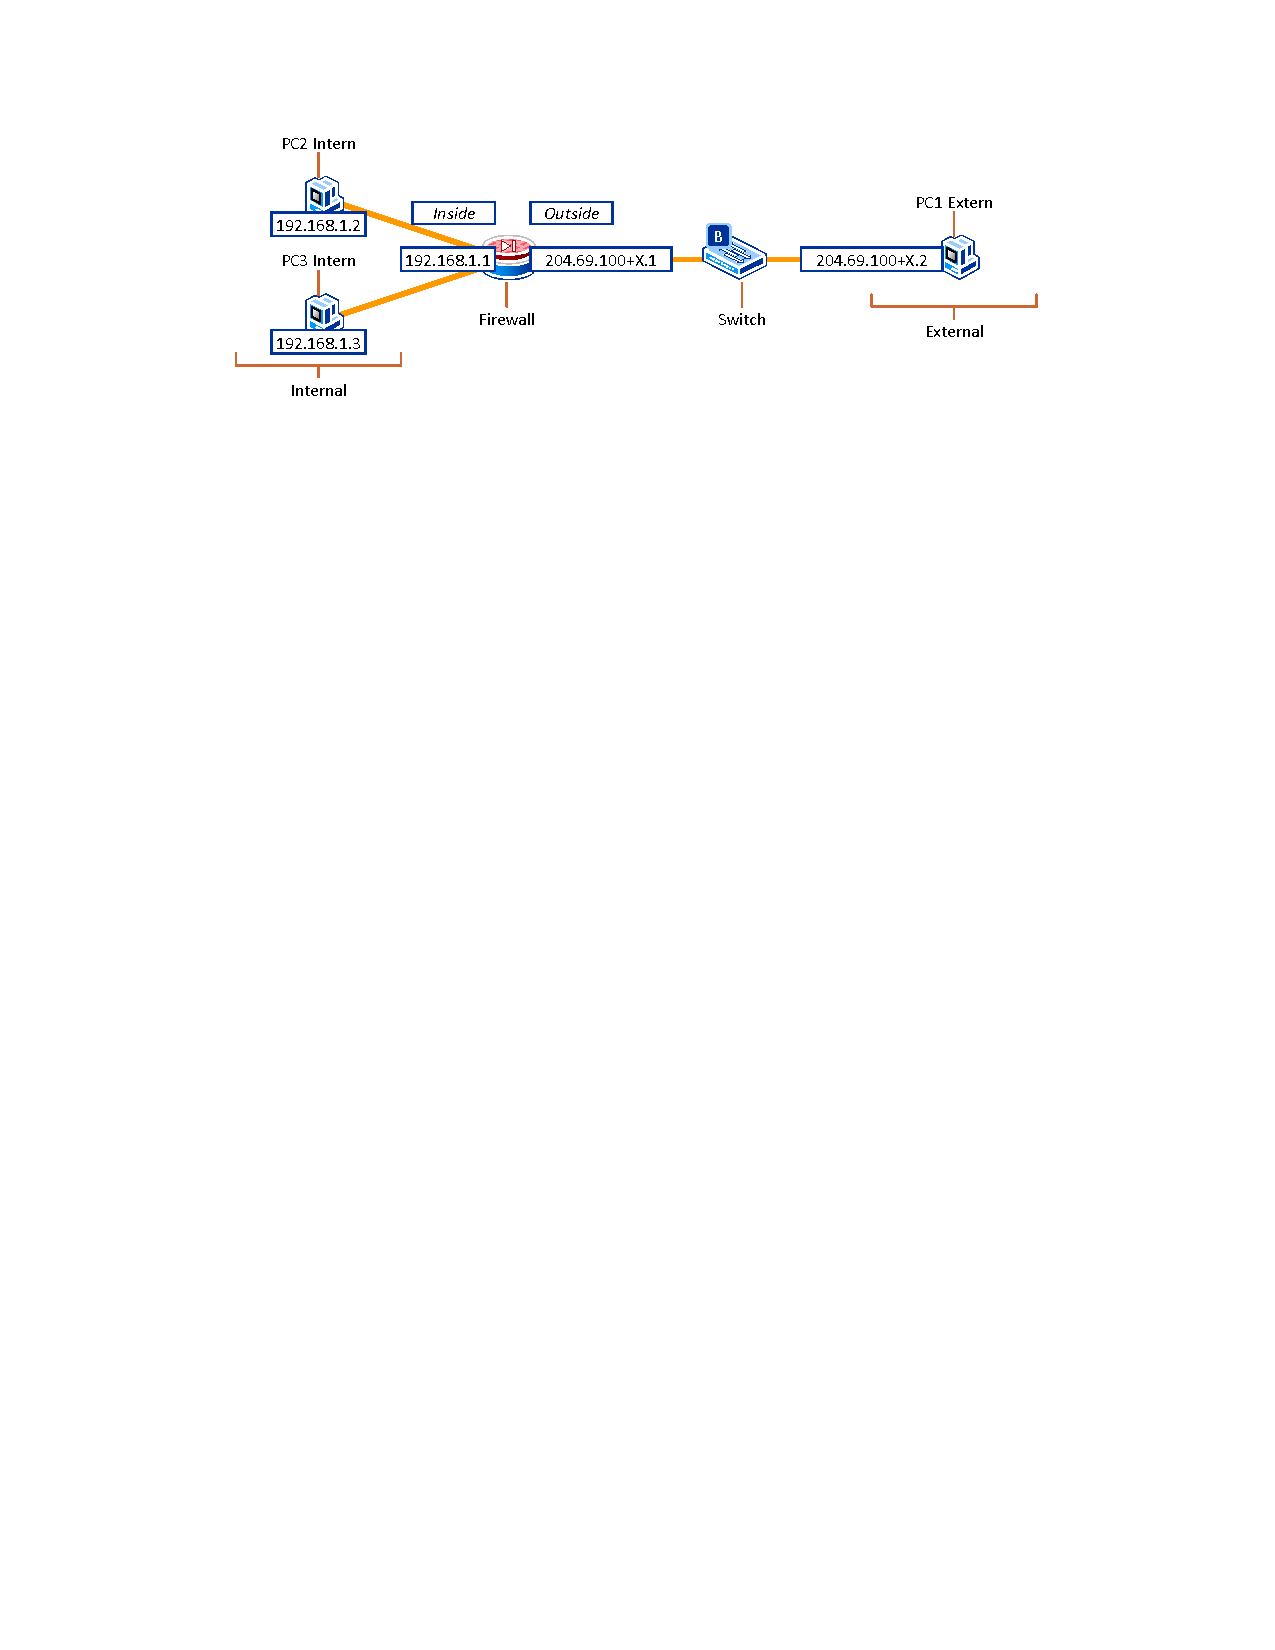
\includegraphics[width=0.9\linewidth]{Figures/Firewall.pdf}
\else
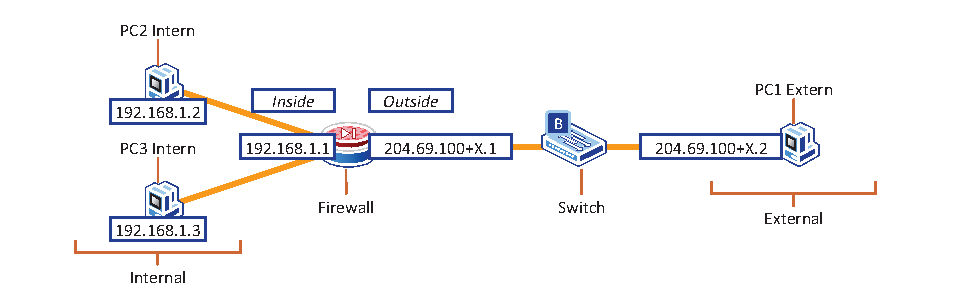
\includegraphics[width=0.9\linewidth]{Figures/Firewall.eps}
\fi
\caption{The network topology for the firewall lab assignment.}
\label{fig:Firewall}
\end{figure}

We shall use the FTP to verify that our network configuration works. Identify the transport layer protocol and the port number for FTP.

\section{Adaptive Security Device Manager (ASDM)}

We will find a shortcut to the \emph{ASDM} application on the desktop. In the case the ASDM is not installed on your computer, open Internet Explorer, disable the proxy and navigate to \url{https://192.186.1.1}, where the default IP address of the firewall is 192.168.1.1. The default username and password are blank. From the firewall's web interface, use the first button to download and install the ASDM on your computer. Once you open the ASDM, use the same IP address, username and password to connect to the firewall.

The CISCO ASA firewalls assign a \emph{security level} to the interfaces. A security level of 100 means the interface is 100\% trusted. A security level of 0 means that the interface is not trusted at all. We shall check the interfaces available and their security level. Discuss the appropriateness of this configuration.

We try to ping between the two computers connected to the internal interfaces.

\begin{center}
\sffamily\small
\begin{tabular}{>{\columncolor{tablegray}}p{15cm}}
\multicolumn{1}{>{\columncolor{tableorange}}l}{Question}\\
With the default configuration of the firewall, does the ping command succeed? Why?\\
\hline
\end{tabular}
\end{center}

\section{Default Configuration of the ASA 5505}

The Cisco ASA use the same OS that the other devices used in the previous assignments, the Cisco IOS. Open the \textsf{Options} \textgreater \textsf{Preferences} menu and check the \textsf{Preview commands before sending them to the device} option. This will show us the equivalent commands that would be used on the console to change the configuration.

Explain which is the default configuration of the firewall.

\begin{center}
\sffamily\small
\begin{tabular}{>{\columncolor{tablegray}}p{15cm}}
\multicolumn{1}{>{\columncolor{tableorange}}l}{Questions and Tasks}\\
Observe and explain the different aspects that can be configured using the icons on the left hand side of the screen.\\
\hline
What is the default configuration of Ethernet 0/0 (outside)?\\
\hline
Why do you thing that the router ships with this configuration?\\
\hline
\end{tabular}
\end{center}

Now, we will change the IP address of the Ethernet 0/0 (\emph{outside}) interface to 204.69.100+X.1. Remember that the X is the group number, and use a /24 network mask. Now we connect the external computer (via switch B) to the \emph{outside} interface. We configure the IP of the external computer to an address of the outside range and we set the firewall's outside address as the computer's default gateway.

\begin{center}
\sffamily\small
\begin{tabular}{>{\columncolor{tablegray}}p{15cm}}
\multicolumn{1}{>{\columncolor{tableorange}}l}{Questions}\\
Can you ping from the outside PC to an inside PC? Why?\\
\hline
What is the difference compared to the previous case?\\
\hline
\end{tabular}
\end{center}

Look at the \textsf{Syslog} from the \textsf{Home} screen to answer this questions.

\section{Firewall}

An alternative configuration option is Telnet. We can enable the Telnet options from the ASDM configuration page using \textsf{Properties} \textgreater \textsf{Device Access} \textgreater \textsf{Telnet}. We have to make sure that we have applied the changes.
Now we connect to the device using a Telnet client and \texttt{cisco} (small letters) as a password.

We try the
\begin{lstlisting}
# who
\end{lstlisting}
command to see who is connected to the firewall.
\begin{lstlisting}
# show run
\end{lstlisting}
to see the running configuration.

\begin{center}
\sffamily\small
\begin{tabular}{>{\columncolor{tablegray}}p{15cm}}
\multicolumn{1}{>{\columncolor{tableorange}}l}{Task}\\
Find information about Telnet and DHCP and explain it.\\
\hline
\end{tabular}
\end{center}

We also try the commands
\begin{lstlisting}
# show interface
\end{lstlisting}
and
\begin{lstlisting}
# show traffic
\end{lstlisting}

\begin{center}
\sffamily\small
\begin{tabular}{>{\columncolor{tablegray}}p{15cm}}
\multicolumn{1}{>{\columncolor{tableorange}}l}{Tasks}\\
Explain the information the previous commands provide.\\
\hline
Discuss the security implications of connecting using Telnet of the console.\\
\hline
\end{tabular}
\end{center}

\section{The Hosts/Networks Table}

In the \textsf{Network Objects/Groups} tab (from the \textsf{Configuration} \textgreater \textsf{Global Objects} page) we can view, edit, add and delete hosts and networks lists defined for every interface. The hosts and networks are organized according to the interface they are connected to (inside/outside). It is recommended to name all the hosts we are managing.

We add the two internal computers by selecting \textsf{Add} \textgreater \textsf{Network Object...}. The network mask is 255.255.255.255, as it is a single host. Add also a corresponding object for the external computer. We apply to save the changes.

\section{Access Rules}

The access rules make it possible to establish security policies as a list of rules. The tables to specify how a computer interacts with another by allowing and denying specific services and protocols. We try to connect from the inside computer to the outside computer and explain the behavior and the default \textsf{Access Rules} (from the \textsf{Configuration} \textgreater \textsf{Security Polivy} page) table for the inside interface.

The rules are examined sequentially until one of the applies. If the first rule applies, the second is not checked. If the first rule does not apply, then the second is checked. The process is repeated until one of the rules applies.

\begin{center}
\sffamily\small
\begin{tabular}{>{\columncolor{tablegray}}p{15cm}}
\multicolumn{1}{>{\columncolor{tableorange}}l}{Question}\\
The last rule is \emph{any to any deny}. Why?\\
\hline
\end{tabular}
\end{center}

The first rule allows traffic from any IP source to any IP destination if the destination interface has a lower security level. If this rule does not apply, the second rule is examined. The second rule always applies and discards the packet.

We shall observe and explain the rules for the traffic arriving to the external interfaces. To understand the rules, we will pay attention to the graphical diagrams offered by the software.

We shall install and configure the FTP server to the external computer. Remember that it is needed to add a folder.

\begin{center}
\sffamily\small
\begin{tabular}{>{\columncolor{tablegray}}p{15cm}}
\multicolumn{1}{>{\columncolor{tableorange}}l}{Question}\\
Is it possible to access the FTP server from the internal computers?\\
\hline
\end{tabular}
\end{center}

Use the rules to deny the access to the FTP server to one of the internal computers and allow access to the other. Observe the log messages to verify that access is being denied. Each time that you change the configuration and try to access to the ftp server, clean the browser cache.

\begin{center}
\sffamily\small
\begin{tabular}{>{\columncolor{tablegray}}p{15cm}}
\multicolumn{1}{>{\columncolor{tableorange}}l}{Task}\\
Include in your report the configuration of the firewall.\\
\hline
\end{tabular}
\end{center}

\section{Translation Rules}

The ASA 5505 supports both network address translation (NAT) which is a one-to-one address translation (one inside to one outside) and port address translation (PAT) which is a many-to-one address translation. Look at the default configuration for the translation rules.

\begin{center}
\sffamily\small
\begin{tabular}{>{\columncolor{tablegray}}p{15cm}}
\multicolumn{1}{>{\columncolor{tableorange}}l}{Questions}\\
How does this configuration affect outgoing traffic?\\
\hline
What is the IP address used after the packets traverse the firewall?\\
\hline
\end{tabular}
\end{center}

\section{Monitoring}

We can use the ASDM for network monitoring. It allows to select the message supervising level. Check the Telnet connections and connected users using the options of the menu on the left. There is also a tool to generate graphs such as traffic, memory and CPU. Look at some of the graphs and enumerate them.

\begin{center}
\sffamily\small
\begin{tabular}{>{\columncolor{tablegray}}p{15cm}}
\multicolumn{1}{>{\columncolor{tableorange}}l}{Task}\\
Include in your report a brief summary of your observations.\\
\hline
\end{tabular}
\end{center}

\section{Case Study}

An enterprise has a C class network 204.69.100+X.0 and wants securely connect their internal network to an external network. The address of the outside firewall interface is 204.69.100+X.1.

In the internal network there is an FTP server with address 192.168.1.4 that needs to be accessed from the outside network using the address 204.69.100+X.4.

The other requirements are that internal users must be able to ping external devices, but not the other way around.

We shall configure the firewall to satisfy the above requirements.

\begin{center}
\sffamily\small
\begin{tabular}{>{\columncolor{tablegray}}p{15cm}}
\multicolumn{1}{>{\columncolor{tableorange}}l}{Task}\\
Explain the changes that we have made and the tests performed to verify the correctness of the configuration.\\
\hline
\end{tabular}
\end{center}


\backmatter
\bibliographystyle{plain}
\bibliography{Lab,Rfc}
\end{document}
